\documentclass{morningstar}
\ctexset{
    section={
        name = {,、},
        format += \raggedright,
        aftername = ,
    },
}
\renewcommand{\theequation}{\arabic{equation}}
\title{使用M/M/m队列系统的云计算动态性能优化}
\major{信号与信息处理}
\phone{19850052801}
\id{221307020006}
\date{2023年01月}
\grade{2022级}
\purpose{《通信网理论》阅读报告}
\author{吉普}
\instructor{李旭杰}

\begin{document}
\setfontformat
\makecover

\clearpage
\startfrontpart
\clearpage

\startmainpart

\showcntitle

\begin{abstract}
    云计算的成功引来了越来越多人和企业的使用。
    一方面,使用云计算降低了成本;另一方面,使用云计算提高了效率。
    由于用户非常关注服务质量(QoS),云计算的性能优化成为其成功应用的关键。
    为了优化云计算中多个请求和服务的性能,我们使用排队论对数据中心服务的各个参数进行了分析和推导。
    然后,通过分析排队系统的性能参数,提出了综合的优化模式、功能和策略。
    最后,我们建立了基于综合优化模式的仿真;我们还将仿真结果与经典优化方法(短时优先和先进先出)进行了比较和分析,
    表明所提出的模型可以优化平均等待时间、平均队列长度和服务客户数量。
\end{abstract}


\section{引言}
云计算是一种提供计算基础设施的新模式,旨在将计算基础设施的位置转移到网络上,以降低硬件和软件资源的管理和维护成本\cite{key1}。 
这种云概念强调将管理、维护和投资从客户转移到提供商。
云计算是一种模型,用于实现无处不在的、方便的、按需的网络访问可配置计算资源共享池(例如网络、服务器、存储、应用程序和服务),
这使得资源可以通过最小的管理成本或与服务提供商的交互来快速提供和释放\cite{key2}。
一般来说,云计算提供了渠道让用户通过网络访问实时可扩展的资源,如文件、程序、数据、硬件、计算和第三方服务。
这些用户通过定制的服务水平协议(SLA)获得计算资源和服务;他们只根据使用时间、使用方式或数据传输量支付费用。
任何SLA管理策略都包含两个完全不同的阶段:合同的协商和履行情况的实时监控。
因此,SLA管理包含SLA合约定义:具有 QoS 参数的基本模式。
在各个方面,QoS是云计算向用户提供服务的基础。 
QoS包括可用性、吞吐量、可靠性和安全性,以及许多其他参数,
但性能指标如响应时间、任务阻塞概率、即时服务概率,以及系统中任务的平均数量\cite{key3},所有这些都可以通过使用排队论这一工具\cite{key4}来确定。
因此,为了满足客户的QoS要求,优化QoS是很重要的。 
由于云计算动态地提供计算资源以满足不同客户对QoS的需求,优化资源利用率将是一项艰巨的任务。
另一方面,一个数据中心拥有大量的物理计算节点\cite{key5};传统的排队分析很少涉及这种规模的系统。
尽管前人的研究已经针对云计算中的关键研究问题提出了几种方法,包括云安全\cite{key6,key7,key8}、隐私\cite{key9,key10}、能源效率\cite{key11}和资源管理\cite{key12,key13,key14},性能优化方面的研究仍然很少。
\par

在本文中,数据中心被塑造成一个服务中心,可以被当成一个具有多任务到达和无限容量的任务请求缓冲区的M/M/m队列系统。 
通过M/M/m排队论,我们推导出各个参数的方程;然后,我们设计了一个优化函数和一个综合优化方法。
仿真结果表明,与短时优先和先进先出的经典方法相比,所提出的优化方法提高了数据中心的性能。
\par

本文的其余部分安排如下。
第2节讨论了性能优化和分析的相关工作。
第3节给出排队模型和优化策略。
我们介绍了模拟设置和模拟结果,然后在第4节中分析和比较了其他经典方法的结果,例如短时优先和先进先出。
在第5节中对我们的工作进行了总结,还概述了未来工作的方向。


\section{相关工作}
尽管云计算引起了研究的关注,但迄今为止只有一小部分工作解决了性能优化问题。
在\cite{key15}中,Li提出了一种面向云计算的差异化服务作业调度系统;
然后,通过分析用户作业的差异化QoS需求,为本系统建立了相应的非抢占式优先级M/G/1排队模型。
他们提供了相应的算法来获取具有不同优先级的每个工作的服务的近似优化值。
在\cite{key16}中,使用云中心模型作为经典开放网络,假设到达时间和服务时间都是指数分布,获得了响应时间的分布。
通过响应时间的分布,发现了任务最大数量、服务资源最小值和服务水平最高值之间的关系。
在\cite{key17}中,他们使用线性预测方法和FPR-R方法从资源利用日志中获取有用信息,使M/M/1排队理论预测方法具有更好的响应时间和更低的能耗。
在\cite{key18}中,他们使用排队模型研究单类服务和多类服务情况下的资源分配问题。
此外,在每种情况下,他们优化资源分配以最小化平均响应时间或最小化资源成本。
\par

此外,一些研究者还进行了性能分析的研究。
在\cite{key19}中,作者提出了一个M/G/m排队系统,表明请求之间的间隔时间是指数分布的;
服务时间是一般分布的,设施节点数量为m。
在另一篇论文\cite{key20}中,作者将云中心建模为一个有单个任务到达和有限容量的任务请求缓冲区的M/G/m/m+r排队系统。
为了评估性能,他们使用了基于变换的分析模型和嵌入式马尔可夫链模型的组合,获得了系统中任务数量和响应时间的完整概率分布。
模拟结果表明,该模型和方法能够准确地预测系统中任务数量的平均值、阻塞概率、及时服务的概率以及响应时间分布的特征,如平均值和标准差、偏度(skewness)和峰度(kurtosis)。
\par

在\cite{key21}中,作者针对云性能管理提出了一种基于排队的分析模型。
在他们的研究中,Web应用程序被建模为队列,虚拟机被建模为服务中心。
他们应用排队理论模型动态地创建和删除虚拟机,以实现扩展和缩减。
\par

在\cite{key22}中,作者分析了云计算中资源配置的一般问题。
为了在不同客户签订不同服务级别协议的情况下支持云资源提供商的资源分配决策,他们使用了带不同优先级类的M/M/C/C排队系统建模了云中心。
他们分析的主要性能标准是可以被解析确定的不同客户类别的拒绝概率。
\par

根据以上分析,我们知道在云计算中已经研究了使用排队理论进行性能评估和分析,但关于性能优化研究很少。
此外,现有研究中已经分别研究了QoS的各个参数,但还没有一项工作同时处理过所有的参数。
在本文中,我们使用具有多个任务到达和无限容量任务请求缓冲的M/M/m排队系统来优化性能。

\section{云计算的排队模型和优化策略}

\begin{figure}[htb]
    \centering
    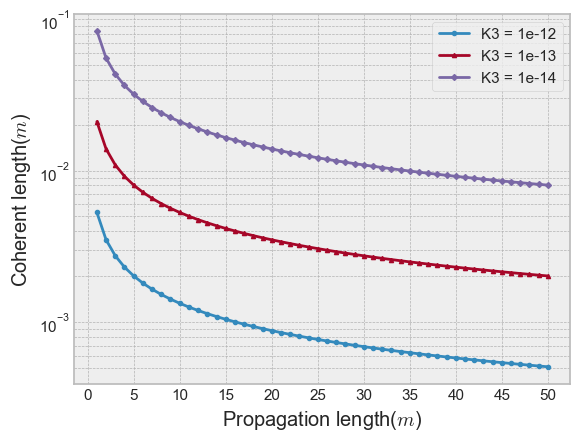
\includegraphics[width=1.0\textwidth]{fig1.png}
    \labeledCaption{云计算服务请求模型图示}
\end{figure}

在云计算中,有很多用户访问服务。
我们将云计算建模如图\ref{云计算服务请求模型图示}所示。
该模型由可以是服务中心的云体系结构组成。
服务中心是全球各地客户的单一访问点。
服务中心是提供商提供的服务资源的集合,用于托管所有用户的应用程序。
每个用户可以根据不同类型的请求申请使用服务并向服务提供商支付一些费用。
\par

云计算提供商建立服务中心供客户使用,如提供多种方式供用户使用的亚马逊。
在本文中,我们使用按需实例。
按需实例允许您按小时计算计算能力的费用,无长期承诺。
这使您免除了计划、购买和维护硬件的成本和复杂性,并将通常的大固定成本转化为小可变成本\cite{key23}。
\par

图\ref{云计算服务请求模型图示}显示的云计算服务模型可以在图\ref{云计算中计算机服务的队列性能模式}中映射为排队模型。
假设有$n$个请求和$m$个服务,且它们都是独立的。
由于连续到达的请求可能来自两个不同的用户,因此到达间隔是一个随机变量,可以在云计算中用指数随机变量来建模。
因此,请求的到达遵循到达率为$\lambda_i$的泊松过程。
调度器队列中的请求分配到不同的计算服务器,调度速率取决于调度器。
假设有$m$个计算服务器,标记为$\text{Service}_1$,$\text{Service}_2$,$\text{Service}_i$以及$\text{Service}_m$;
服务速率为$\mu_i$。
所以,总的到达率为$\lambda = \sum_{i=1}^n \lambda_i$,总的服务率为$\mu = \sum_{j=1}^m \mu_i$。
排队论已经证明了在$\lambda / \mu < 1$的情况下,系统是稳定的。
服务率跟到达率一样,遵循泊松过程。
因此,M/M/m排队模型适用于云计算模型。

\begin{figure}[htb]
    \centering
    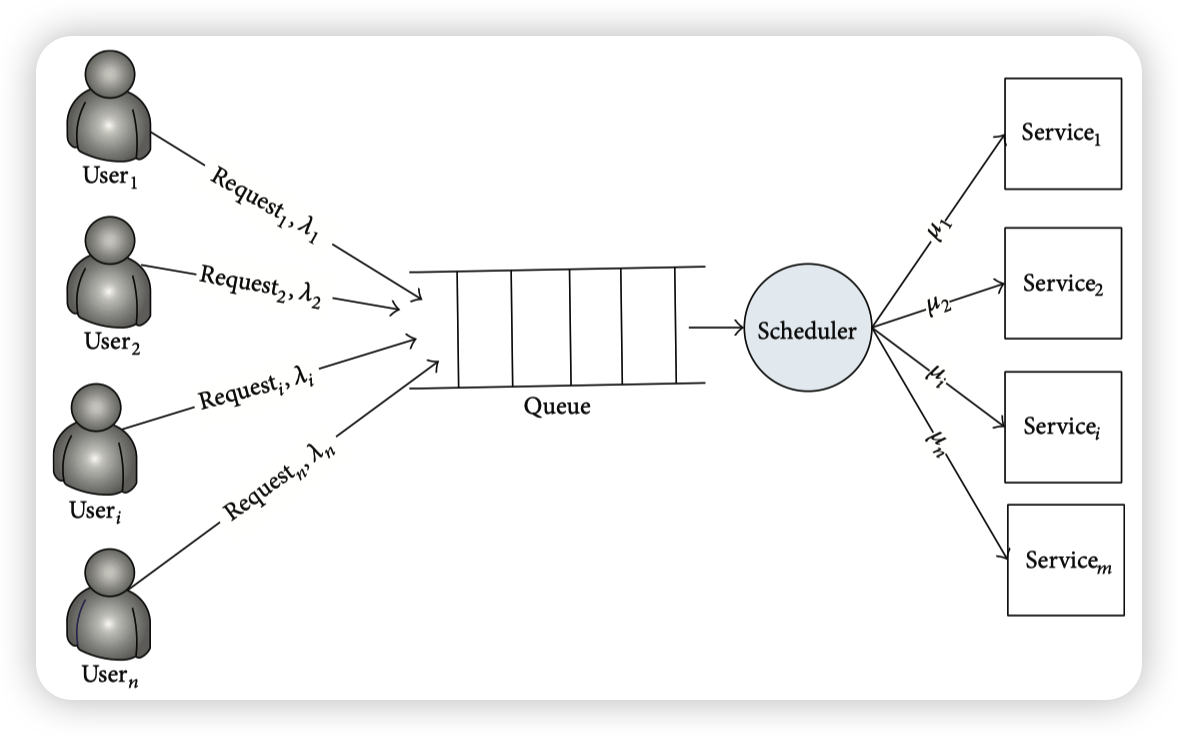
\includegraphics[width=1.0\textwidth]{fig2.png}
    \labeledCaption{云计算中计算机服务的队列性能模式}
\end{figure}

\subsection{状态平衡方程}
\begin{figure}[h]
    \centering
    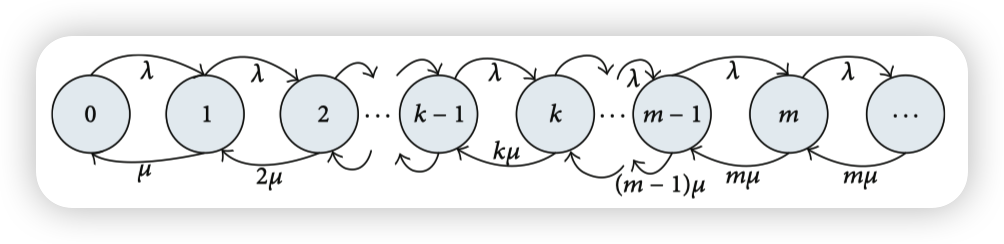
\includegraphics[width=0.95\textwidth]{fig3.png}
    \labeledCaption{状态转移概率图}
\end{figure}

由于客户的请求来自世界各地,云计算可以提供无限的服务,因此客户的来源和排队模型的数量是不受限制的。
系统的状态集合为$E=\{0,1,2,...\}$;
因此这些平衡方程也可以由图\ref{状态转移概率图}中的M/M/m状态转移图来描述。
\par

当状态为$k(0 \le n \le m)$,有$n$个服务在忙,其余的$m-n$个服务空闲;
当状态为$k(m \le n \le \infty)$,有$m$个服务在忙,其余的$n-m$个客户在等待。
设 $\rho = \lambda /(m\mu)$,假定满足稳定条件$\rho < 1$,则根据M/M/m队列有以下状态平衡方程:

\begin{equation}
    \begin{aligned}
    & p_1=m \rho p_0, \\
    & p_2=\frac{m^2}{2 !} \rho^2 p_0, \\
    & p_3=\frac{m^3}{3 !} \rho^3 p_0, \\
    & p_m=\frac{m^m}{m !} \rho^m p_0, \\
    & \ldots \\
    & p_{m+r}=\frac{m^m}{m !} \rho^{m+r} p_0 .
    \end{aligned}
\end{equation}

\noindent 因此,可得通式:
\begin{equation}
    \label{eq:2}
    \begin{gathered}
    p_n=\frac{m^n}{n !} \rho^n p_0, \quad 0 \leq n<m, \\
    p_n=\frac{m^m}{m !} \rho^n p_0, \quad n \geq m .
    \end{gathered}
\end{equation}

为了获得$p_0$,我们累加公式\ref{eq:2}的两边,因为$\sum_{n=0}^{\infty}p_n = 1$,
我们可以获得关于$p_0$的等式,可以得到$p_0$的解为:
\begin{equation}
    p_0=\left(\sum_{n=0}^{m-1} \frac{\rho^n}{n !}+\frac{\rho^k}{k !} \times \frac{k}{k-\rho}\right)^{-1} .
\end{equation}


\subsection{平均队列长度,延迟和等待时间}
\label{平均队列长度,延迟和等待时间}

为了评估和优化性能,我们应该推导参数的方程。
首先,我们定义以下符号:

\begin{itemize}[leftmargin=4em]
    \item $L_s$ 是一个随机变量,代表系统中客户的总数(包含在队列中等待的和正在被服务的);
    \item $L_q$ 是一个随机变量,代表在队列中的客户数(不包含正在被服务的);
    \item $N_s$ 是一个随机变量,代表正在被服务的客户数;
    \item $W_s$ 是一个随机变量,代表系统中的延迟(这包含用户排队和被服务的时间);
    \item $W_q$ 是一个随机变量,代表用户在队列中的等待时间(不包含用户被服务的时间);
    \item $\tau$ 是一个随机变量,代表服务时间。
\end{itemize}

根据上面的符号定义,我们可以得到:
\begin{equation}
    \begin{aligned}
    & E\left[L_s\right]=E\left[L_q\right]+E\left[N_s\right], \\
    & E\left[W_s\right]=E\left[W_q\right]+E[\tau] .
    \end{aligned}
\end{equation}
很显然,
\begin{equation}
    E[\tau]=\frac{1}{\mu} .
\end{equation}

为了获得M/M/m队列的$E[N_s]$,我们对系统使用Little公式。
如果我们只考虑系统中的服务器而不考虑服务器外的等待室,可以发现,由于没有阻塞带来的损失,系统的到达率就是$\lambda$,
而平均服务时间就是$E[\tau] = 1 / \mu$。因此,根据Little公式,处于忙绿的服务器数可以表示为:
\begin{equation}
    E\left[N_s\right]=\frac{\lambda}{\mu}=\rho
\end{equation}

为了获得$E[L_q]$,我们假设两个相互排斥和详尽的事件 \{ $q \ge m $ \}, and \{$q < m$\},我们可以得到:
\begin{equation}
    \begin{aligned}
    E\left[L_q\right]= & E\left[L_q \mid q \geq m\right] P(q \geq m) \\
    & +E\left[L_q \mid q<m\right] P(q<m) .
    \end{aligned}
\end{equation}


为了获得$E[L_q | q \ge m ]$,我们可以发现当$q \ge m$时,M/M/m队列就可以等价于一个服务速率$m\mu$的M/M/1队列;
所以,这个M/M/1队列的平均队列长度等于$\rho / (1- \rho)$,其中$\rho = \lambda/ (m\mu)$,因此:
\begin{equation}
    E\left[L_q \mid q \geq m\right]=\frac{\rho / m}{1-\rho / m}=\frac{\rho}{m-\rho} .
\end{equation}

\noindent 由于$E[L_q|q<m] = 0 $并且$P(q\ge m)= C_m(\rho)$,我们可以得到:
\begin{equation}
    E\left[L_q\right]=C_m(\rho) \frac{\rho}{k-\rho} .
\end{equation}


\subsection{优化策略和优化算法}
在云计算中,数据中心有很多服务。
在\ref{平均队列长度,延迟和等待时间}中,我们已经讨论了M/M/m队列系统的很多参数。
队列中用户数量的参数为$L_s$,$L_q$和$N_s$;在这三个参数中,$L_q$起主导作用,
因为正在被服务的用户数量由系统中服务器的数量决定,而$L_q$取决于服务器的性能。
我们选用利用率,平均时间和等待被服务的用户数量作为优化参数。
基于排队论系统的任务调度和性能优化模型如图\ref{基于队列系统的任务调度和性能优化模型}所示。
\begin{figure}[htb]
    \centering
    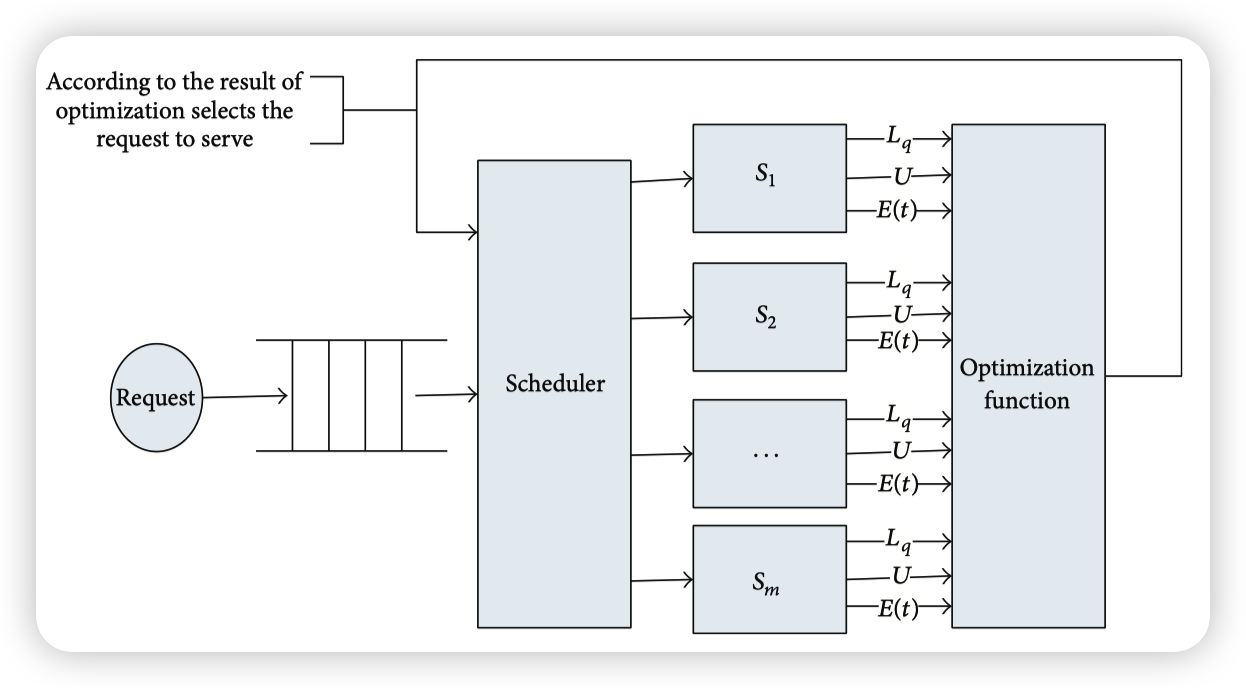
\includegraphics[width=1.0\textwidth]{fig4.png}
    \labeledCaption{基于队列系统的任务调度和性能优化模型}
\end{figure}

优化策略如下:
所有请求都会到达调度器,根据优化函数的结果选择将请求发送到服务器。
优化函数的输入参数是云计算中每个服务器的时间平均值、利用率和等待客户总数。
设$p_i$是$i$个用户被选择并执行的概率,$t_i$是$i$个用户的服务时间,因此,平均时间$E(t)$如下:
\begin{equation}
    E[t]=\sum_{i=1}^m p_i * t_i
\end{equation}

\noindent 为了获得优化结果,并保证负载均衡,优化函数如下:
\begin{equation}
    \mathrm{fcn}=\alpha * E[t]+\beta * L_q+\chi * U_i
\end{equation}

\noindent 其中,$\alpha$, $\beta$ 和 $\chi$ 是可以通过训练获得的系数,而$E[t]$,$L_q$和$U$ 分别是平均时间,队列中的用户数 和 每个服务器的利用率。
利用率$U_i = \lambda_i/ \mu_i$,其中$\lambda_i$是优化函数选择的客户到达率,$\mu_i$是服务器$S_i$的服务率。
优化函数根据填充参数计算函数值,然后按升序排序。
调度器根据优化函数的结果选择服务器来执行服务。
根据最优策略,优化算法在算法中进行描述。
\par

根据最优策略,优化算法在算法\ref{优化算法}中进行描述。
% \begin{algorithm}
%     %      
%     % \SetKwFunction{getvalueE}{getvalueE}

%     \Input{request_list, server_list} 
%     \Output{server_number} 
%     \BlankLine
% \end{algorithm}

\begin{algorithm}[H]
    \setstretch{1}
    \SetKwData{server}{server}
    \SetKwInOut{Input}{input}
    \SetKwInOut{Output}{output}
    \Input{request\_list, server\_list}
    \Output{server\_number}
    % \KwIn{request\_list, server\_list}
    % \KwOut{server\_number}
    \BlankLine
    \For{server in server\_list}{
        $E(t)$ = getvalue$E$(server\_number)\;
        $L_q$ = getvalue$L_q$(server\_number)\;
        $U$ = $\lambda_i$ / $\mu_i$\;
    }
    \For{for server in server\_list}{
        function\_value = $\alpha * E(t)_i + \beta * (L_q)_i + \chi * U$\;
    }
    \emph{ascending sort of the valued of function\_value}\;
    \emph{getting the index of the first function\_value}\;
    \emph{scheduler schedules the request to the select\_server}\;
    \labeledCaption{优化算法}
\end{algorithm}



\section{仿真与结果分析}

\subsection{仿真设置}

为了验证我们的优化策略的性能,我们使用MATLAB的离散事件工具。
所有实验都在 AMD Phenom II X4 B95 3.0 GHz,2 G RAM 的微软 Windows XP 环境下进行测试,所有实验都在 MATLAB R2009b 中实现。
我们按照亚马逊标准的按需实例将请求分为四类。

请求的到达时间间隔遵循指数分布,并且平均到达率为\{ $\lambda_1 = 30$, $\lambda_2 = 20$, $\lambda_3 = 15$, $\lambda_4 = 12$ \}。
服务也遵循指数分布,且平均服务率为 \{ $\mu_1=3$, $\mu_2=2.4$, $\mu_3=2$, $\mu_4=1.71$ \}。
优化函数的系数分别是\{ $\alpha = 0.1$, $\beta = 0.4$, $\chi = 2$ \};总的测试时间是一天(1440分钟),服务器的数量是\{4, 20, 40, 60, 80\}。

\subsection{仿真结果和分析}

我们将我们的优化方法作为合成优化(SO)的优先队列。
为了比较和分析优化策略的性能,我们使用经典的短时优先的优先级队列和先进先出(FIFO)排队策略作为测试度量。
我们使用优先队列块来实现基于优化策略的排队策略,并将两种优先排队策略的性能与 FIFO 排队策略进行比较。
\par

\begin{table}[htbp]
    \centering
    \labeledCaption{平均等待时间}
    \begin{tabular}{lcccc}
    \hline
    Service number      & \makebox[60pt]{FIFO}                  & \makebox[60pt]{SSF}                   & \multicolumn{2}{c}{\makebox[100pt]{SO}}    \\
    \hline
    4                   & 705.2                 & 114.8                 & \multicolumn{2}{c}{688.2} \\
    20                  & 475.5                 & 43.42                 & \multicolumn{2}{c}{304.6} \\
    40                  & 166.6                 & 47.4                  & \multicolumn{2}{c}{0.59}  \\
    \multirow{2}{*}{60} & \multirow{2}{*}{2.64} & \multirow{2}{*}{2.64} & \makebox[50pt]{48}         & \makebox[50pt]{0.025}        \\
                        &                       &                       & 52         & 0.0010       \\
    80                  & 0.06                  & 0.06                  & 60         & 0            \\
    \hline
    \end{tabular}
\end{table}
\begin{table}[htbp]
    \centering
    \labeledCaption{平均队列长度}
    \begin{tabular}{lcccc}
    \hline
    Service number & \makebox[60pt]{FIFO} & \makebox[60pt]{SSF} & \multicolumn{2}{c}{\makebox[100pt]{SO}}   \\
    \hline
    4                   & 892.3                 & 892.3                 & \multicolumn{2}{c}{890.6} \\
    20                  & 607.3                 & 607.3                 & \multicolumn{2}{c}{398.1} \\
    40                  & 206.2                 & 206.2                 & \multicolumn{2}{c}{0.76}  \\
    \multirow{2}{*}{60} & \multirow{2}{*}{3.39} & \multirow{2}{*}{3.39} & \makebox[50pt]{48}  & \makebox[50pt]{0.032}    \\
                        &                       &                       & 52         & 0.0013       \\
    80                  & 0.077                 & 0.077                 & 60         & 0            \\
    \hline
    \end{tabular}
\end{table}
\begin{table}[htbp]
    \centering
    \labeledCaption{服务客户量}
    \begin{tabular}{lccc}
    \hline
    Service number & \makebox[80pt]{FIFO} & \makebox[80pt]{SSF}  & \makebox[80pt]{SO}   \\
    \hline
    4              & 101  & 101  & 102  \\
    20             & 667  & 667  & 1083 \\
    40             & 1517 & 1517 & 1848 \\
    60             & 1848 & 1848 & 1848 \\
    80             & 1848 & 1848 & 1848 \\
    \hline
    \end{tabular}
\end{table}

首先,我们测试了服务器数量分别为\{4, 20, 40, 60, 80\}时的平均等待时间。三种策略的结果如表\ref{平均等待时间}所示。
根据表\ref{平均等待时间},当服务器数量为4和20时,SSF的平均等待时间最少;
但是,当服务器数量为40,60和80时,SO策略的平均等待时间最少。
当服务器少的时候,许多用户被迫在队列中等待;另一方面,短时服务首先被完成,短时服务的服务时间小于其他策略的服务时间。
因此,SSF策略的平均等待时间是最佳的。
然而,当服务增加时,即服务器数量为40,60和80时,SO策略综合优化了利用率,平均等待时间和平均队列长度,并使每个服务器能力发挥最佳效果。
因此,平均等待时间比其他策略短。
与SO策略相比,当服务增加时,SSF和FIFO策略无法顾全每个服务器的利用率和队列长度。
因此,某些服务器可能无法完全运行,而其他服务器可能过载,导致更长的平均时间。
\par

另一方面,表\ref{平均队列长度}和表\ref{服务客户量}显示了三种策略的平均队列长度和服务客户数。
上面两张表表示SO的平均队列长度和服务客户数量比其他两种策略更好。
尽管 SSF 的平均等待时间在服务率为 4 和 20 时很好,但 SSF 策略的平均队列长度和服务顾客数量并不比 SO 策略更好。
原因如下:服务器太少时,无法为到达的顾客提供足够的服务,大多数顾客不得不排队等候。
当服务人员增加时,SO 可以优化平均等待时间、平均队列长度和利用率。
因此,SO 能够获得实现更多的用户服务,平均队列长度更短。
\par

\begin{figure}[h]
    \centering
    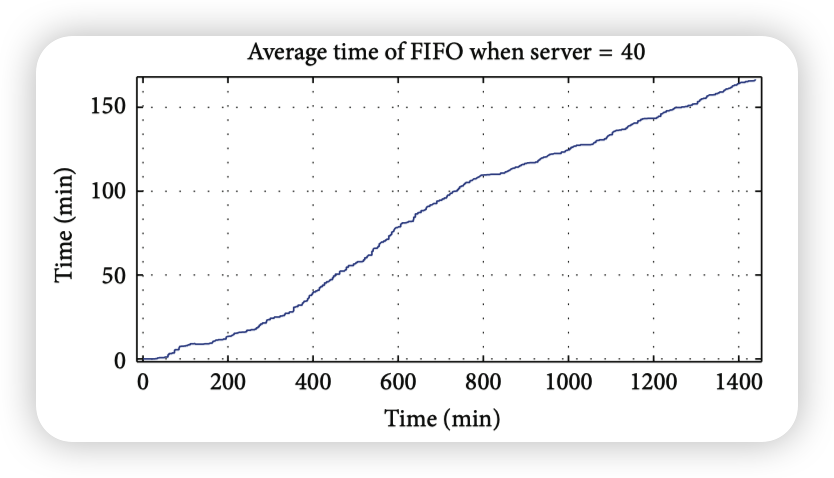
\includegraphics[width=0.88\textwidth]{fig5.png}
    \labeledCaption{平均等待时间[FIFO]}
\end{figure}

为了清楚地展示队列的平均等待时间,当服务器数为40时,三种策略的曲线图在图\ref{平均等待时间[FIFO]}、\ref{平均等待时间[SSF]}和\ref{平均等待时间[SO]}中给出。
当顾客请求服务太多而FIFO服务策略无法提供足够的服务时,图\ref{平均等待时间[FIFO]}显示平均等待时间几乎是随着时间的推移而线性增加的。
\par

虽然平均等待时间也有所增加,但与图\ref{平均等待时间[FIFO]}相比,图\ref{平均等待时间[SSF]}明显有所改善。图\ref{平均等待时间[SO]}表明,随着时间的推移,平均等待时间先上升后下降。
原因如下:由于用户增加,首先服务器的利用率没有显著提高,因此等待时间会增加;随着服务器利用率的增加,等待时间也会减少。

\begin{figure}[h]
    \centering
    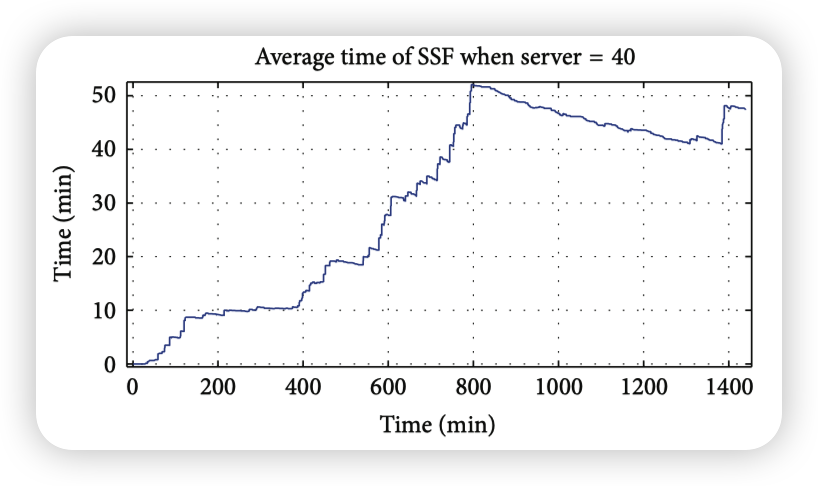
\includegraphics[width=0.88\textwidth]{fig6.png}
    \labeledCaption{平均等待时间[SSF]}
\end{figure}
\begin{figure}[h]
    \centering
    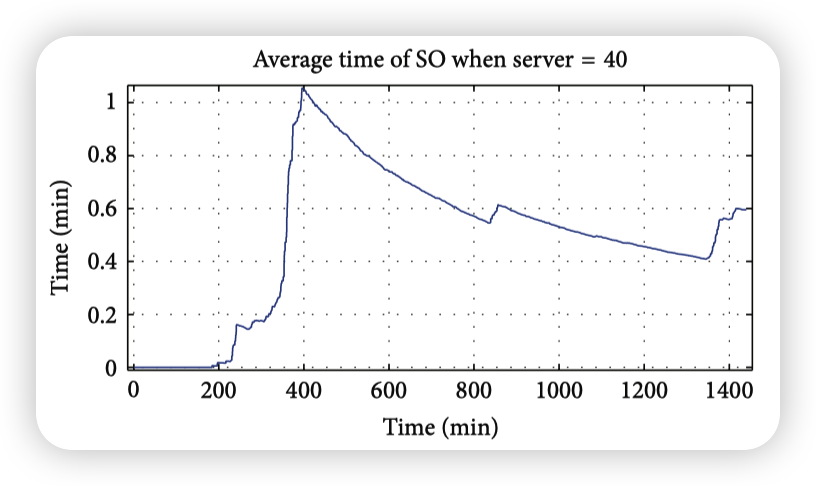
\includegraphics[width=0.88\textwidth]{fig7.png}
    \labeledCaption{平均等待时间[SO]}
\end{figure}



\clearpage
\section{总结与展望}

我们研究了在云计算中优化性能的方法,并给出了评估服务的参数。
通过模拟,我们可以回答以下问题:
(1) 对于给定的服务数量和客户到达率,可以获得多少水平的QoS?
(2) 对于给定的QoS要求和客户到达率,用多少服务器能够满足QoS?
(3) 对于给定的服务器数量和客户到达率,有多少客户能够获得服务?
在本文中,为了分析云计算中服务的性能,我们提出了一种排队模型,并开发了一种综合优化方法来优化服务性能。
我们进一步进行了模拟以验证我们的优化方法。
模拟结果表明,所提出的方法可以减少等待时间和队列长度,并使更多的客户获得服务。
为了在真实的云计算环境中评估所提出的系统,我们计划通过扩展真实的云平台(如OpenStack)来实现它。
此外,如果将云计算建模为M/M/G,则可以适用于不同的服务时间。我们将来会研究这方面。
目前,在云计算中,数据中心的电力消耗非常巨大;
因此未来研究的另一个方向是优化性能和能耗。
此外,这项工作具有社会重要性,它不仅可以降低正在进行的运营成本,还可以减少二氧化碳。


\vspace{1em}
\addbib{paper.bib}


\startappendix

\section{仿真结果}
\begin{itemize}
    \item \textbf{`code/distribute`}: 请求的分布图
    \item \textbf{`code/record`}: 请求的信息记录表
    \item \textbf{`code/waitTime`}: 平均等待时间的时序图
    \item \textbf{`code/result.xlsx`}: 平均等待时间、平均队列长度、服务客户量
\end{itemize}

\section{仿真代码}
\subsection{main.py}
\inputminted[linenos,fontsize=\zihao{-6},mathescape,numbersep=5pt,frame=lines,firstnumber=8,highlightlines={8,10}]{python}{code/main.py}
\subsection{lib.py}
\inputminted[linenos,fontsize=\zihao{-6},mathescape,numbersep=5pt,frame=lines,firstnumber=8,highlightlines={8,10}]{python}{code/lib.py}


\end{document}




